\chapter{Probabilistic Model}
\label{chap:statistical_model}

\lettrine{I}{ntroduction} into this chapter\dots

\pagebreak

\section{Time series representation and \aclp{gp}}
\label{sec:time_series_analysis}

\todo[inline]{introduction to GP. search over all functions. emphasize the aspects of it that we are using it for, but also a bit generally why it's good for ML. compare it to other interpolation/extrapolation methods. if makes sense, explain to what kind of data it suits.}

%\subsection{Covariance functions (kernels)}
\subsection{Kernel building and tuning}
\label{subsec:covariance_functions}

\todo[inline]{current information taken from \url{http://scikit-learn.org/stable/modules/gaussian_process.html}. in the introduction add the reference(s) mention at the end of this page.}
\todo[inline]{also, there was a very detailed thesis/paper about kernels, check if there are more good details there}

Kernels (also called \textit{covariance functions} in the context of \acp{gp}) are a key component \acp{gp}, as they define the statistical relationship between the input values.
In general, they represent describe the similarity $k(x, x')$ between each pair of input points, so that $k(\cdot, \cdot)$ determines how similar the outputs $y_*$ and $y_*'$ will be. 
More formally, a covariance function can be described as $\mathcal{K}(u, v) = \phi(u) \cdot \phi(v)$, where $\phi(\cdot)$ is a function that maps the input vectors into a transformed feature space.
Which function to use is a key question when modeling using a \ac{gp}, as it determines the behavior of the model and the quality of the predictions it will be able to make.
Naturally, some assumptions and decisions regarding the data must be made when choosing a kernel.
A kernel's parameters are optimized to achieve functions that better fit the data, the consistency of the resulted functions is measured using log maximum likelihood.

Since convergence analyses usually refer to the \textit{difference} between values in different production (as opposed to the values themselves), stationary kernels are more suitable for fitting \ac{gp} to them, as they are shaped by the distances between each pair of data point rather than merely their absolute values.
%That is, they fulfill $k(x_1, x_2) = k(x_1 - x_2)$.
%This list only covers a small subset of common covariance functions.
%Further kernels include the exp-sine squared, dot-product, linear, and more.
%\putref{put 2 references about kernels, or only 1 is the first is used above}
Kernels can also be chained using multiplication or addition to combine characteristics of multiple kernels.
Multiplication-based kernels are maximized when all of its kernel factors yield high values, whereas
Addition-based kernels, are maximized when any of their addend kernels yield a high value.
%For example, multiplying a linear kernel by a periodic one will result in functions that are \textit{both} periodic \textit{and} with increasing amplitude as they move away from the origin.
For the modeling presented here, an additive kernel is used with constant, RBF, and noise terms (see \crefrange{eq:constant_kernel}{eq:RBF_kernel}).
The RBF term determines the general shape of the curve (see example in \cref{fig:RBF_prior_posterior}), the constant term enables shifting of the curve if necessary, and the noise term adds degrees of freedom in case the curve cannot completely fit the input signal.

The definitions of the used kernels are as follows:

\begin{description}
	\item[Constant kernel -- ]
	This is a simple kernel that assigns the same value for all input pairs.
	Since by itself it does not offer a lot of characteristic to the covariance function, it is usually used as part of a product kernel, where which it scales the magnitude of the other factors, or as part of a sum kernel, in which it modifies the mean of the Gaussian process.
	It has a single parameter, the constant value, and it is defined as 
	%
	\begin{equation}
		\label{eq:constant_kernel}
		k_{constant}(C, x, x') = C\forall x_1, x_2,
	\end{equation}
	\eqname{Constant kernel}
	%
	where $C$ is the constant value parameter.
	
	\item[Noise kernel -- ]
	is a kernel used for capturing unexplained variation in the data, i.e., noise.
	It is typically based on the constant kernel as part of a sum kernel, in which it explains the noise component of a signal.
	In this context, the constant parameter is tuned to estimate the noise level.
	This is determined by
	%
	\begin{equation}
		\label{eq:noise_kernel}
		k_{noise}(\{noise\_level\}, x, x') =
		\begin{cases}
		C_{noise\_level}, & if\quad x_1 = x_2\\
		0, & otherwise,\\
		\end{cases}
	\end{equation}
	\eqname{Noise kernel}
	%
	where $noise\_level$ equals the variance of the noise found in the input signal.
	
	\item[Radial-basis function (RBF) kernel --]
	also known as \emph{squared exponential kernel}, the RBF kernel is a stationary kernel with one parameter, \emph{lengthscale} $l > 0$.
%	 which can either be a scalar (isotropic variant of the kernel) or a vector with the same number of dimensions as the inputs x (anisotropic variant of the kernel).
	This kernel typically results in generally smoothed functions, with the lengthscale being associated with the long-term smoothness and degree of variability on the time dimension.
	The RBF kernel is defined as
	%
	\begin{equation}
		\label{eq:RBF_kernel}
		k_{RBF}(\{\ell\}, x, x') = \sigma^2 exp\left(\frac{\lVert x_1 - x_2 \lVert ^2_d}{2\ell^2}\right),
	\end{equation}
	\eqname{Radial basis function (squared exponential) kernel}
	%
	where $\lVert x_1 - x_2 \lVert$ is the Euclidean distance between two $d$-dimensional input points and $\sigma^2$ is a scalar factor that determines the average distance of your function away from its mean.
	\cref{fig:RBF_prior_posterior} shows prior and posterior examples of the RBF kernel.
	
%	\item[Rational quadratic kernel]
%	This kernel can be seen as a scale mixture (infinite sum) of RBF kernels with different length scales.
%	Therefore, \acp{gp} priors with this kernel expect to see functions which vary smoothly across many length scales.
%	It has two parameters: length scale $l > 0$ and scale mixture $\alpha > 0$.
%	The parameter $\alpha$ determines the relative weighting of large-scale and small-scale variations.
%	When $\alpha$ $\lim$ $\inf$, the RQ kernel is identical to the SE kernel, as described by
%	
%	\begin{equation}
%		\label{eq:RQ_kernel}
%		k_{RQ}(\{\sigma, \alpha, \ell\}, x, x') = \sigma^2 \left( 1 + \frac{\lVert x_1 - x_2 \lVert ^2}{2\alpha \ell^2} \right)^{-\alpha}.
%	\end{equation}
%	\eqname{Rational quadratic kernel}
\end{description}

\subsection{Data interpolation using kriging}
\label{subsec:interploating_data_using_kriging}
	
\begin{figure}[t]
	\centering
	\subfigure[RBF kernel prior ($length scale = 1$)]
		{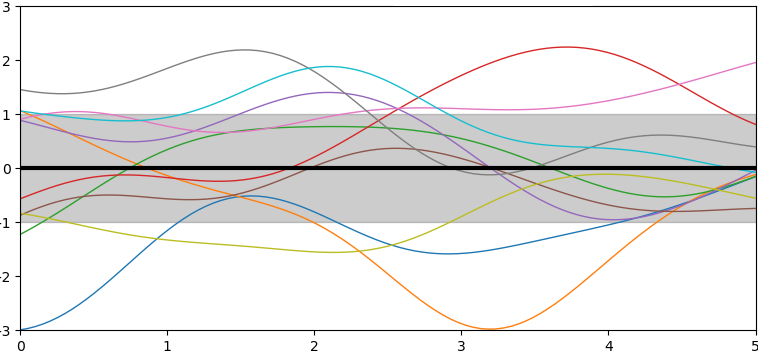
\includegraphics[width=0.45\textwidth]{RBF_prior}
	\label{fig:RBF_prior}}
	\hfill % no empty line here to avoid staring a new paragraph (figures will be vertically aligned)
	\subfigure
	[RBF kernel posterior ($length scale = 0.279$)]
	{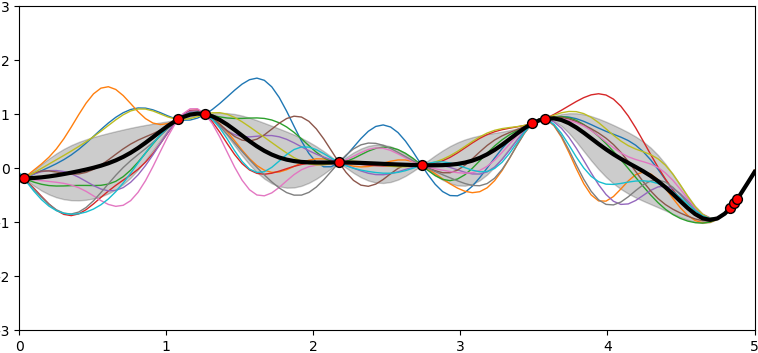
\includegraphics[width=0.45\textwidth]{RBF_posterior}
	\label{fig:RBF_posterior}}
	\caption[Prior and posterior of RBF kernel]
		{\hspace{-0.18cm}\footnotemark\ 
		Prior and posterior distributions of an RBF kernel with mean zero, resulted in a Gaussian process $\mathcal{GP}\left( 0 (\vec{x}), \Sigma(\vec{x}) \right)$.
		Each color line stands for a drawing (prediction) from the prior and posterior distributions, and the thicker black line shows the overall mean of the distributions.
		The red circles are the known data points on which the kernel was optimized to fit, and the gray areas mark the \SI{95}{\percent} confident intervals above and below the overall mean.
		The length scale parameter (in parentheses) determines the length of the \enquote{wiggles} of the functions}
	\label{fig:RBF_prior_posterior}
\end{figure}
\footnotetext{adapted from \url{https://scikit-learn.org/stable/_images/sphx_glr_plot_gpr_prior_posterior_001.png}}

As also motivated in \cref{subsec:limitations_of_did,subsec:temporal_analysis}, artificially splitting interactions into a fixed, pre-determined number of parts to measure accommodation results in a partial view on the process.
To avoid that, some interpolation method is required, with the goal of yielding a more general behavior based on the observed productions.
This allows analysis on continuous series of values instead of point-by-point comparison, where the temporal gaps between data points might be greatly unbalanced.
One way of achieving that, using \ac{loess}, is shown in \cref{fig:hds_dds_time_pitch}.
A more evolve approach is presented here, where a speaker's vocal behavior is described as a distribution of functions that match the accumulated \textit{evidence} from the speaker's productions.

\citet{Galvez2020unifiying}\\ % compare to the rather simplistic (and naive) approach taken here (based on TAMA) -- can refer to some of the specific methods there, specifically that they also use area under curve difference
\citet{Kousidis2008towards}\\ % original TAMA paper. read again, but seems like it's glorified moving average. say that my appraoch actually learns the curve of the speaker and doesn't just interpolate, which allows continuous predictions and more evolve description.
\citet{Kousidis2009monitoring}\\ % another TAMA paper, with an a bit more concrete example

Kriging (or \textit{\acl{gp} regression}) is an interpolation method that gives an optimally fitted and unbiased prediction of intermediate values.
\todo{references for a few fields where it is used?}
Since this method fits a function distribution over the data, it not only yields mathematically more likely values, but also provides a curve that describes the characteristics of the interpolated curved, as opposed to more naive methods like linear interpolation or smoothing spline.
Another advantage of this method is that it yields a \textit{distribution over functions} rather than specific values.
Therefore, an infinite number of suitable values can be drawn from one fitted kernel and their likelihood can be evaluated.
Such interpolation is illustrated in \cref{fig:RBF_posterior}, where each line represents a mean regression prediction drawn from the posterior distribution based on the given data points.

This method was applied on the dataset presented in \cref{sec:vacc}.
For simplicity, only the interactions in solo condition were used.
The functions prediction for a each speaker can be described by
%
\begin{equation}
	\label{eq:gp_function_prediction}
	f_*(\vec{x}) = \mathcal{GP}(\mu_{speaker}, \Sigma_*),
\end{equation}
\eqname{Function predicted using a fitted Gaussian process}
%
where $\mu_{conv}$ is the mean feature value of a single speaker and $\Sigma_*$ is the fitted additive covariance function described in \cref{subsec:covariance_functions}.
It is important to note that the mean is not zeroed (as usually done in \ac{gp} regression) to maintain the original input values for the subsequent steps.
The kernel was initialized with the priors $C = 1$, $lengthscale = 1$, and no assumptions regarding noise level.
The search boundaries for the RBF and noise components were $1 < lengthscale < 100$ and $\num{1e-4} < \xi < 10$, respectively, with a maximum of six optimization iterations. % the initial one plus five allowed restarts (n_restarts_optimizer parameter in code)
\todo[inline]{make sure these numbers are up to date}
\todo[inline]{write about how datapoints where selected from each turn to represent points of change}
With the fitted kernel, a continuous prediction can be made for each speaker over the entire conversation time span.
\Cref{fig:gp_vacc} shows an example of \ac{gp} predictions for one of the conversations. % 20171121A_Calendar_01 was used
%
\begin{figure}[t]
	\centering
	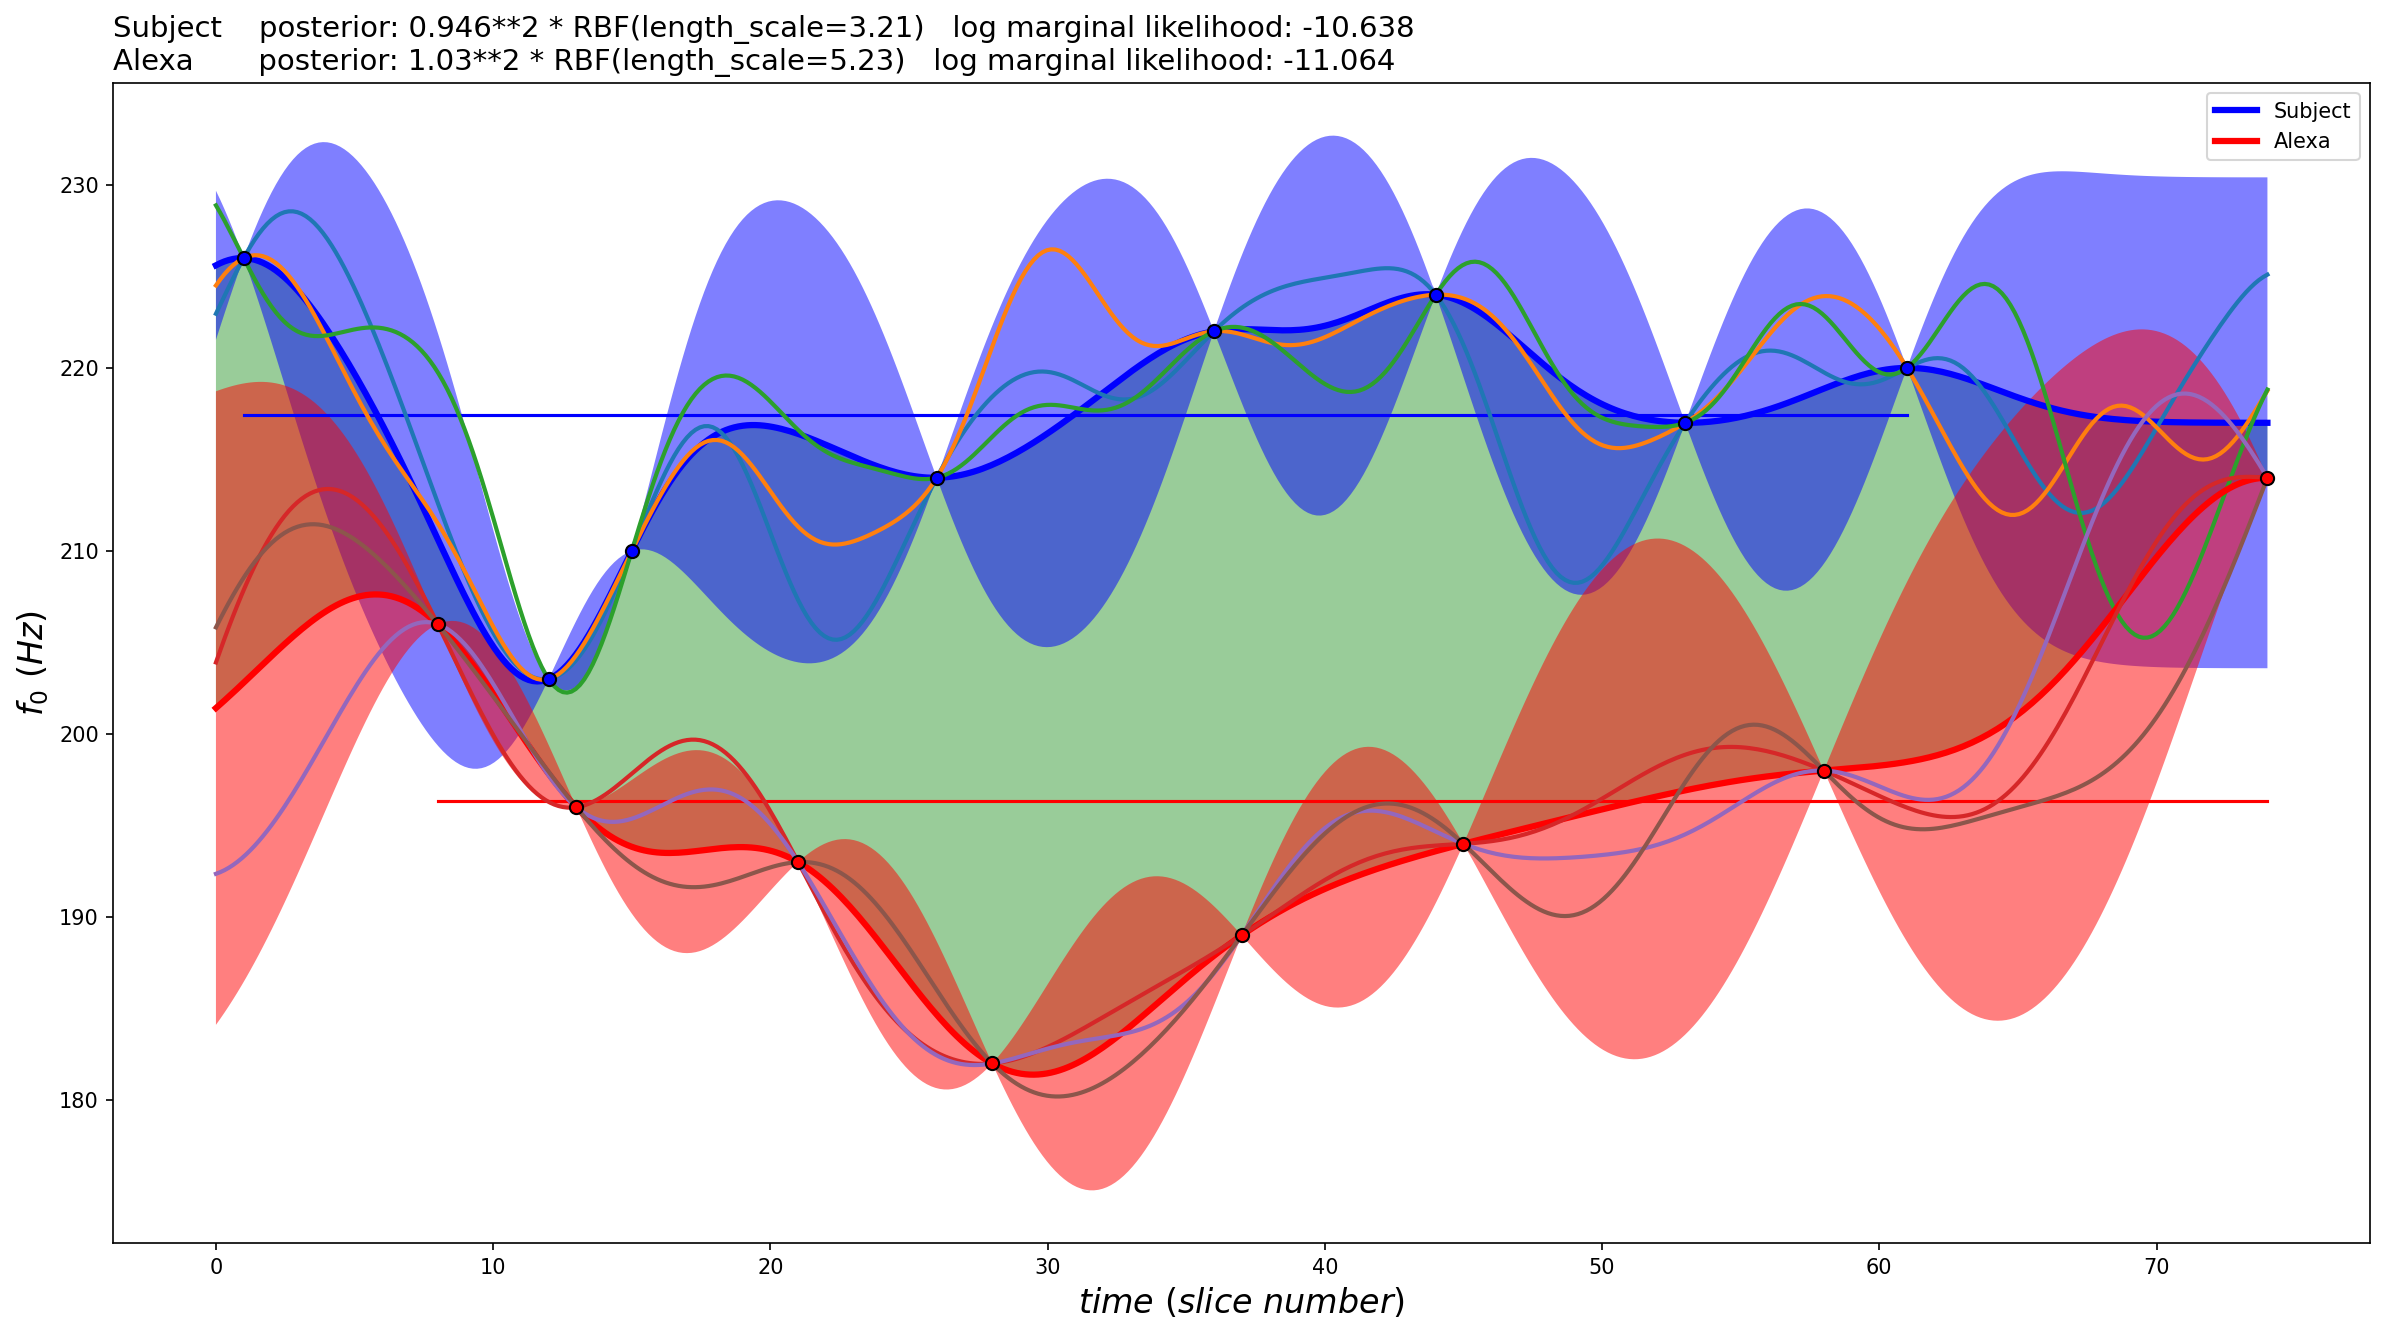
\includegraphics[width=\textwidth]{GP_VACC_with_draws}
	\caption[Gaussian process regression on conversation with Alexa]
		{Gaussian process regression for an interaction of a subject with Alexa.
		 The thick blue and red lines show the predictions' mean.
		 The additional lines around the means are randomly drawn functions from the fitted kernel representing potential variational output.
		 The colored areas around the means lines show the \SI{95}{\percent} confident interval for the distributions of the same color.
		 The straight horizontal lines indicate the overall mean of each speaker's productions.
		 The posterior parameters and the log marginal likelihoods of the fitted distributions are stated at the top.}
	\label{fig:gp_vacc}
\end{figure}

\section{Marking degrees of change}
\label{sec:measuring_changes}

Once a regression line is drawn for each speaker from their respective distributions, the differences between the speakers' productions can be measured.
Furthermore, due to the higher temporal resolution, more fine-grained degrees of change over time can be calculated as well.
The differences are calculated by the subtracting the trapped areas between the two regression lines (see \cref{fig:gp_vacc})
%
\begin{equation}
	f_{diff} \equiv\Delta\vec{x}_* =
	\int_{\vec{x}_i}^{\vec{x}_{j}}\mu_{f_*subject} -
	\int_{\vec{x}_i}^{\vec{x}_{j}}\mu_{f_*alexa}
\end{equation}
%
and the directional derivatives of the resulted delta line to measure the degree of change
%
\begin{equation}
	\nabla\Delta\vec{x}_*' = \frac{d}{dx}f_{diff}
\end{equation}
%
along the difference line.
\Cref{fig:diff_and_derivatives} demonstrates this on the same conversation from \cref{fig:gp_vacc} using the mean predictions of each speaker.
%
\begin{figure}[t]
	\centering
	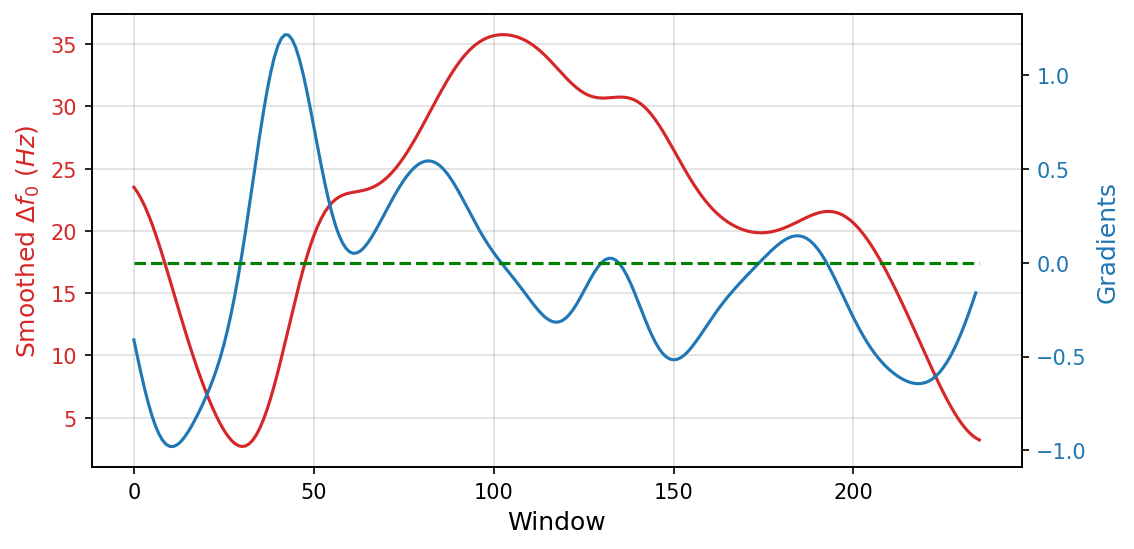
\includegraphics[width=\textwidth]{diff_and_derivatives}
	\caption[Continuous integral differences and derivatives in a \acl{hci}]
		{Continuous integral differences (red line) and their corresponding derivatives (blue line) of speakers' productions in a conversation.}
	\label{fig:diff_and_derivatives}
\end{figure}
%
For building a generative model as described in \cref{sec:accommodation_as_a_lm,clustering_and_incremental_generation}, the changes must be marked with pre-defined labels.
To that end, the derivative values were translated into a continuum of change ranging from \textit{divergence} to \textit{convergence}.
Based on this continuum, a discrete scale can be defined.
The more categories this discrete scale offers, the more specific the behavior descriptions can be.
\Cref{fig:cont_disc_scales} shows this process for a discrete scale of three categories: divergence, no (major) change, and convergence.
%
\begin{figure}[t]
	\centering
	\subfigure[Continuous scale]
		{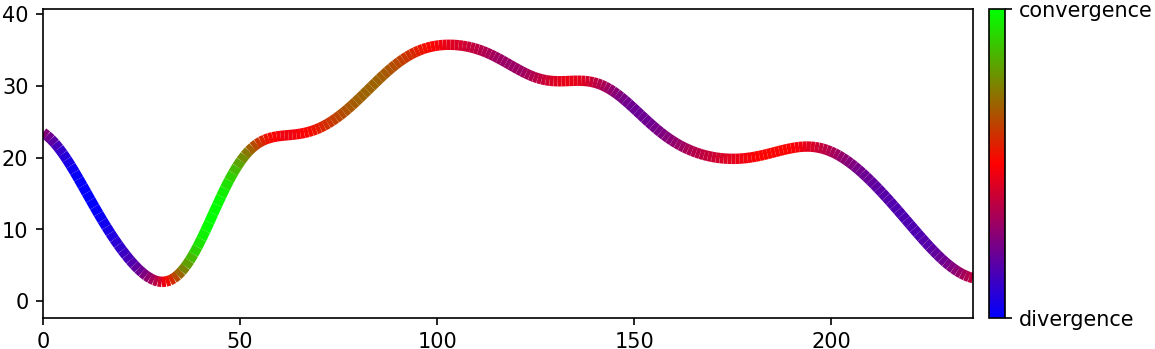
\includegraphics[width=0.47\textwidth]{cont_scale}
	\label{fig:continuous_scale}}
	\hfill
%	\vspace{-1cm}\hfill\hspace{-1cm}{\hbox{\LARGE $\Longrightarrow$}}\hfill
	\subfigure[Discrete scale]
		{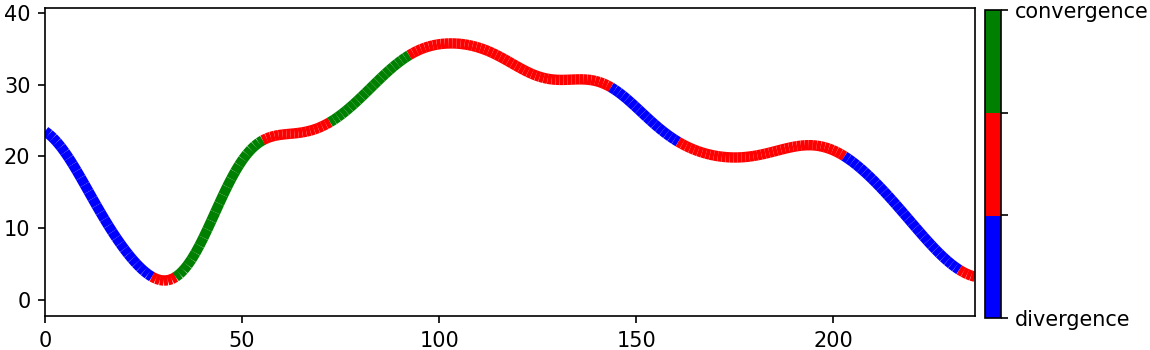
\includegraphics[width=0.47\textwidth]{discrete_scale}
	\label{fig:discrete_scale}}
	\caption[Continuous and discrete scales for labeling degrees of change]
		{Continuous and discrete color-coded scales for labeling degrees of change in a conversation.}
	\label{fig:cont_disc_scales}
\end{figure}
\todo[inline]{more details regarding how the discrete categories are defined}


\section{Accommodation as a language model}
\label{sec:accommodation_as_a_lm}

\todo[inline]{say that an n-gram language model has the advatage of ver other methods like markov chains that it takes time (history) into account (as opposed to only the last state), which I claim to be important in accommodation (and refer to one of the places where this is explained)}

\subsection{Dimensionality reduction and symbolic representation}
\label{subsec:dim_reduction_and_symbolic_rep}

\subsection{Sequence extraction and probabilities}
\label{subsec:word_extraction_and_seq_prob}

[\ldots] similar distributions were found for all $n$ size up to half the size of an whole interactions.

\section{Clustering and incremental variational generation}
\label{clustering_and_incremental_generation}

\begin{figure}[t]
	\centering
	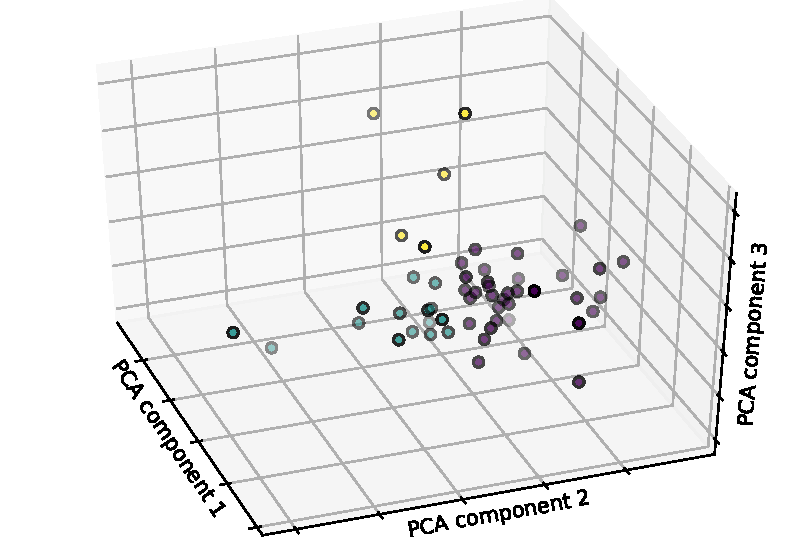
\includegraphics[width=\textwidth]{3d_clustering}
	\caption[3D \ac{knn} clustering of degrees of change \ac{pca} components]
		{}
	\label{fig:knn_clustering}
\end{figure}

\todo[inline]{1-2 intro sentences that both bottom-up and top-down approaches are shown here and each has its useful insights (which??)}


Since the \ac{paa} representations created in \cref{subsec:dim_reduction_and_symbolic_rep} can be arbitrarily long and high dimensional, they are reduced here to their $n$ first \ac{pca} components for the purposes of visualizing their clustering.
The k-nearest neighbors algorithm was used for clustering.
the process was performed for 2, 3, and 5 clusters using the first 2 or 3 first \ac{pca}, with the combination of 3 clusters and 3 components performing the best on average.
% on average since kNN is not deterministic and was run multiple times
The result is shown in \cref{fig:knn_clustering}.

\todo[inline]{what else can be said about the kNN clustering?}

\todo{need references for PCA and KNN?}

\begin{landscape}
	\begin{figure}[t]
		\centering
		\hspace*{-4cm}
		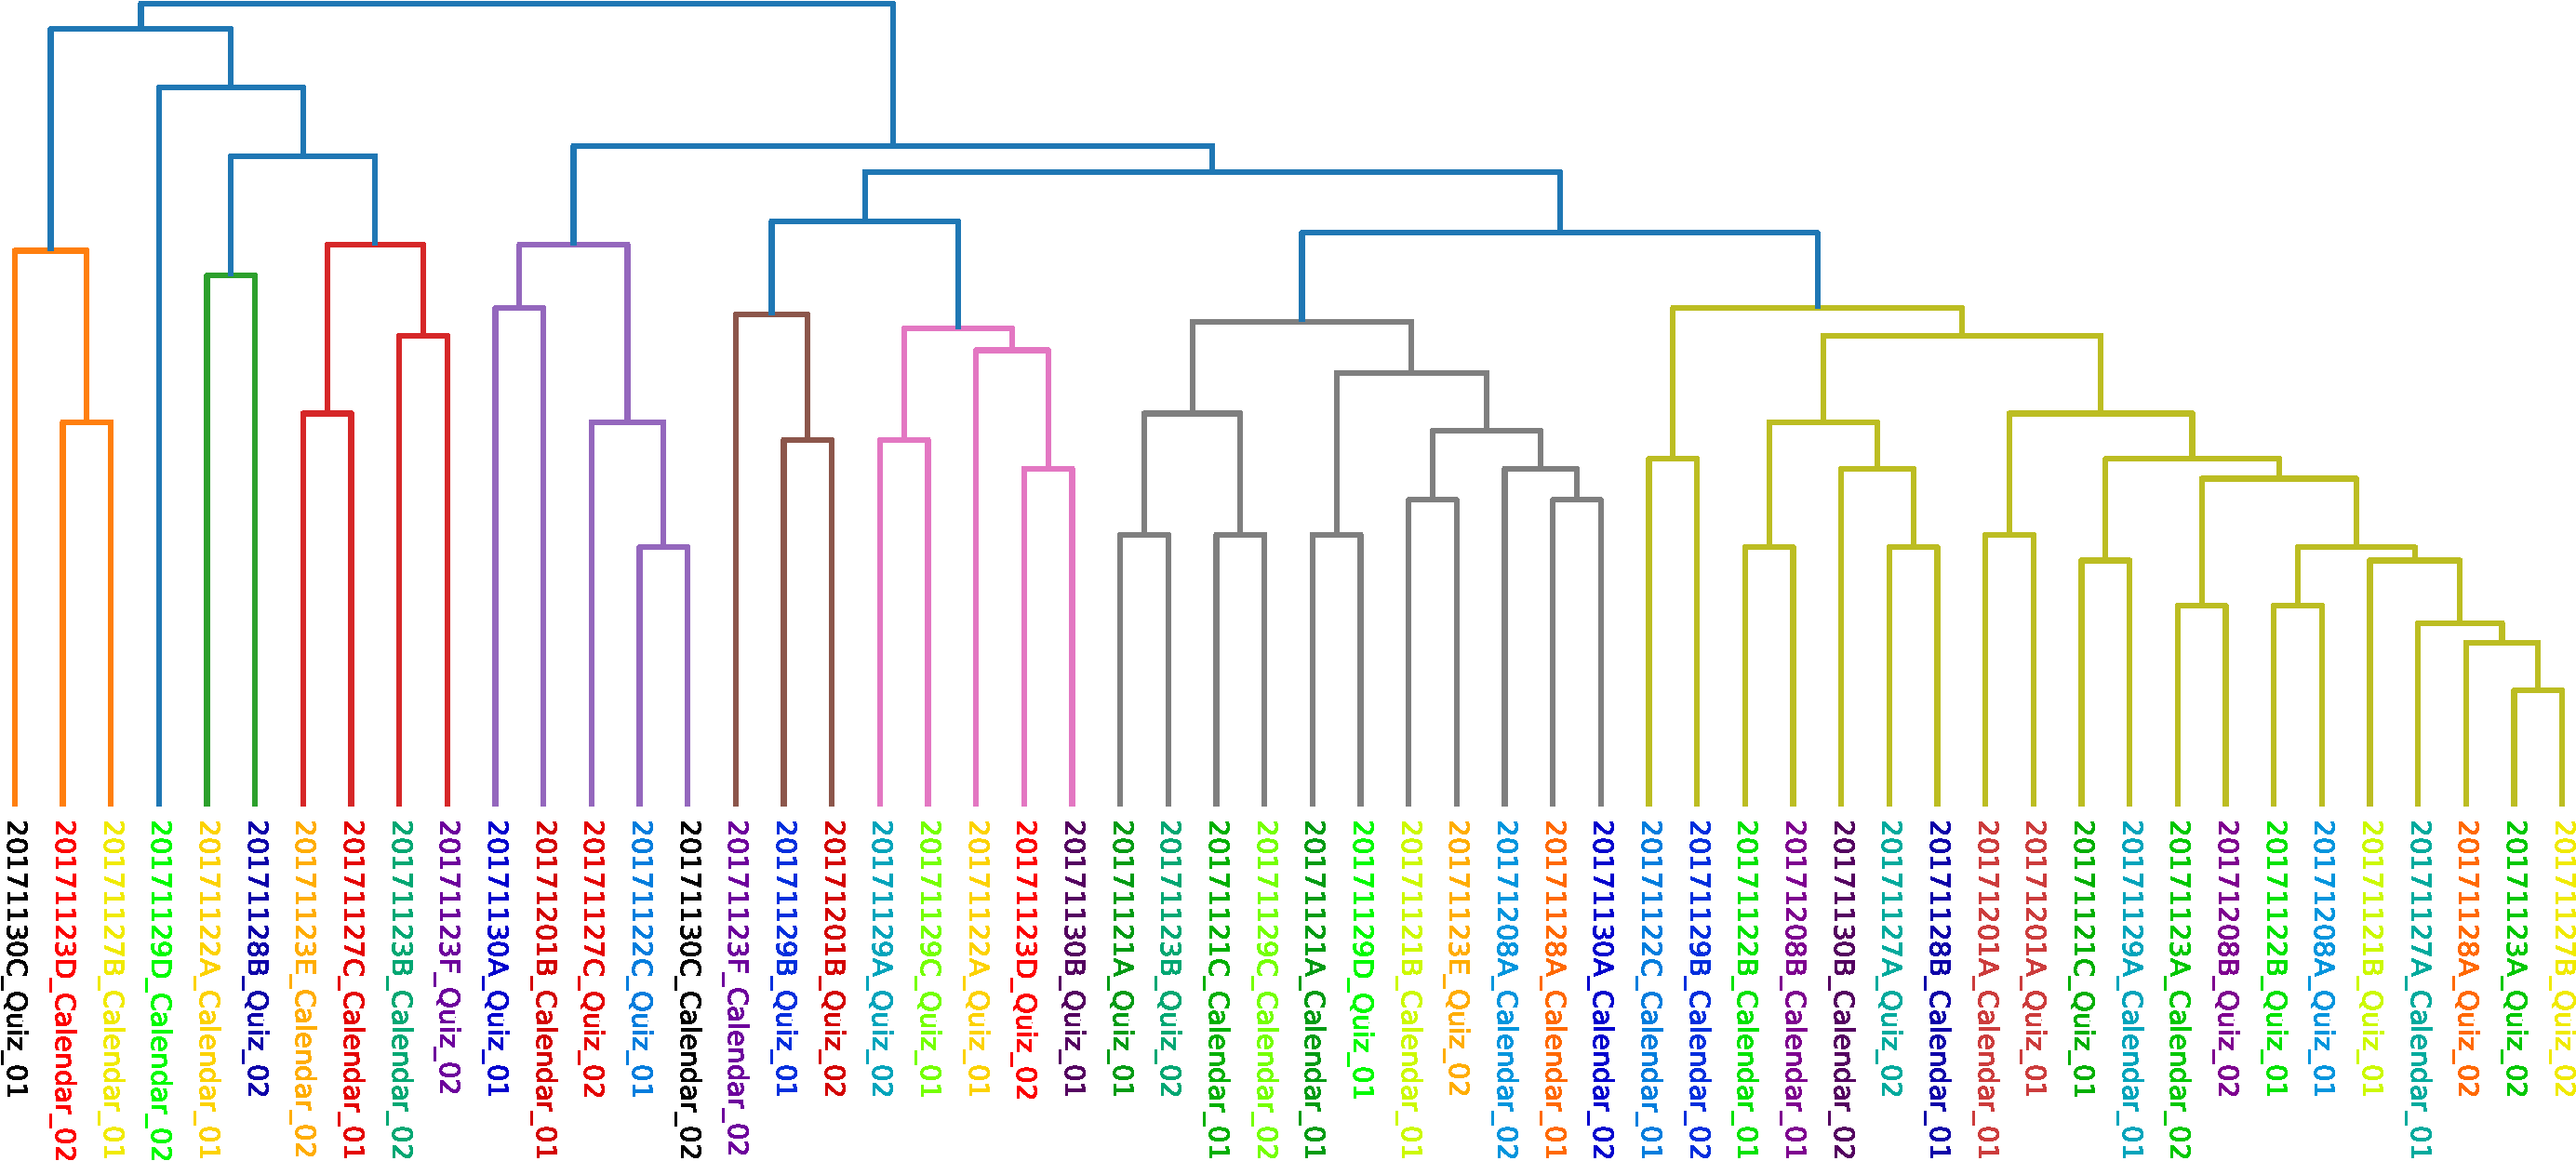
\includegraphics[width=1.7\textwidth]{paa_dist_dendrogram}
		\caption[Dendrogram of time series representation of interactions distances]
			{Dendrogram of the time series \ac{paa} representations of the solo condition interactions based on complete-link distances.
			 Each cluster is represented by a different color of lines.
			 Blue lines connect pairs of clusters that are most similar to each other, and similarly pairs of the closest subsequent sub-cluster and eventually leaves are connect directly to each other.
			 Each leaf represent the interaction indicated by its label.
			 Labels of the same color mark interaction with the same subject (two interactions per subject).
			 The leaf and cluster colors are \emph{not} related.
			 The leaves are order horizontally by their distance from left to right, so that the leaves of interactions that are more similar to each other (both inter- and within-cluster) are positioned closer.
			 For example, the two interactions of subject \emph{20171201A} (12\textsuperscript{th} and 13\textsuperscript{th} leaves from the right) are the closet to each, as they are positioned together and within the same smaller sub-cluster.}
		\label{fig:paa_dist_dendrogram}
	\end{figure}
\end{landscape}

\todo[inline]{if this really works decently, refer to this section when describing variational vocal behavior as one of the levels for accommodative SDS}

While top-down clustering can uncover general grouping of elements, bottom-up hierarchical clustering can reveal structural relations between them and measure their degrees of similarity.
With numeric values assign to the degrees of changes along an interaction via the the \ac{paa} representations created in \cref{subsec:dim_reduction_and_symbolic_rep}, the distances between the 54 interactions can be measured and compared.
The calculation was done using \emph{complete link} (a.k.a.\ farthest point algorithm).
This kind of linkage is supported by the assumption that there are more general behavior patterns beyond the individual differences, as it searches the most dissimilar (and hence principally all) interactions in neighboring clusters and not only the closest one.
This method also allows using the entire \ac{paa} sequences.
\Cref{fig:paa_dist_dendrogram} shows the bottom-up distance clustering based on this linkage. 
Although, unsurprisingly, no definite order emerges, some general trends can be seen regarding the similarity between interactions of the same subject.
As the leaves are ordered horizontally based on their overall similarity, the distances between their positions be utilized to determine each subject's behavior consistency.
The average distance of the population is 16.5, far from the maximal possible average of 27.
% This is the maximal possible average, since this is when each interaction is half of the population away from its pair.
% With the largest possible distance between two leaves being 53, the space can be divided into three bins of 18 (rounded up).
Dividing the space into three equal bins of \enquote{short}, \enquote{medium}, and \enquote{long} distances shows that 15, 10, and 2 interactions fall into these bins, respectively.
Moreover, this distribution has median of 17 and the second tertiles at 19, far from the 
Such skewed distribution indicates that interactions of the same speaker tend to be relatively similar in terms of accommodation trends, regardless of any other factor (interaction length, task, order, and other factors used in \cref{chap:speech_variations_in_hhci}).
Notably, the two interactions of one participant, 20171201A, even have the minimal possible distance of 1 between them (leaves (12\textsuperscript{th} and 13\textsuperscript{th} in \cref{fig:paa_dist_dendrogram}) and they are located together in the smallest sub-cluster.

\todo[inline]{if it's not too much work, calculate how many subjects are in the same-color cluster}.